%!TEX root = ../../../memoria.tex
\section{Control de Acceso}

%TODO: Agregar comentarios iniciales
Control de acceso limita las acciones directas de un usuario, así como que programas pueden ejecutarse \cite{sandhu1994access}
 
%Meteor Accounts
%Meteor Accounts is a complete user account system that you can drop into your application. With one line of code, you can have login, logout, account creation, email validation, password recovery, and login with OAuth providers like Facebook or Twitter.
Existe un sistema completo de cuentas de usuarios el cual permite hacer \loginCPT(\refFigura{figure:account:sign_in_ui}), \logoutCPT(\refFigura{figure:account:log_out}), creación de cuentas (\refFigura{figure:account:create_account}), y recuperacion de contraseña(\refFigura{figure:account:reset_password}). Aunque en estricto rigor, la recuperación de contraseña momentaneamente corresponde a una contraseña aleatoria generada por la aplicación y enviada al correo.


\subsection{Creación de cuenta de un usuario}

La creación de una cuenta se ha pensado realizando la menor cantidad de acciones posibles( ver \refFigura{figure:architecture:accounts:new:form}). Agregar acciones innecesarias puede significar que los usuarios desistan y dejen el sitio\cite{online_goodgui_org}.

\begin{figure}[H]
	\centering
	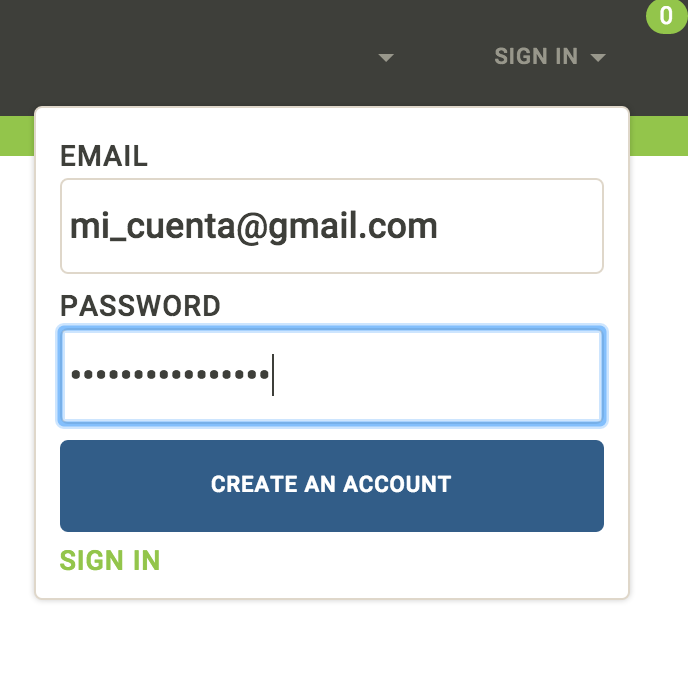
\includegraphics[width=0.4\textwidth]{figuras/architecture/accounts/new/form.png}

	\caption{Formulario de creación de una cuenta.}
	\label{figure:architecture:accounts:new:form}
\end{figure}


El formulario de creación tiene ciertas restricciones las cuales deben cumplirse para la creación exitosa de una cuenta. La \reftabla{tab:architecture:accounts:new:form} resume todas las restricciones del formulario. En la \refFigura{figure:architecture:accounts:new:send_error} pueden verse los errores que muestra el formulario para guiar al usuario.

\begin{table}[H]
    \centering
	\begin{tabular}{ |l|c||l| }
		\hline Campo & Requerido & Restricción \\ \hline
		\multirow{2}{*}{\textit{Email Address}} &  \multirow{2}{*}{\checkmark}
				& - Debe ser un \email válido. \\ 
			& 	& - El \email no debe pertenecer a un usuario previamente ingresado.\\ \hline
		\multirow{2}{*}{\textit{Password}} 		&  \multirow{2}{*}{\checkmark}	
				& - Debe tener al menos 6 caracteres \\ 
			& 	& - Debe contener al menos un número o símbolo. \\ \hline
	\end{tabular}
 	\caption{Resumen restrincciones para formulario creación de cuentas de usuario.}
    \label{tab:architecture:accounts:new:form}
\end{table}

\subsection{Autenticarse}

Al igual que el formulario de creación de usuario, el formulario de autenticación tiene solo dos campos (\refFigura{figure:architecture:accounts:signin:form}).

\begin{figure}[H]
	\centering
	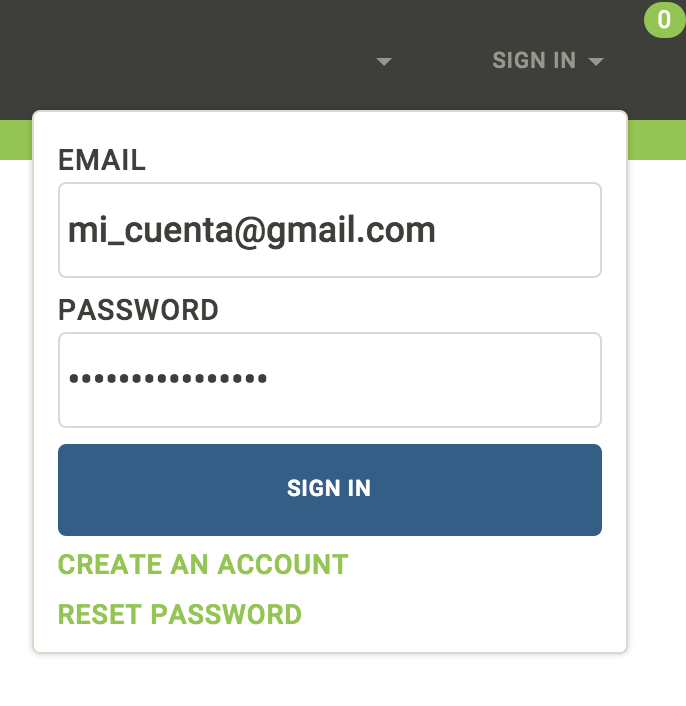
\includegraphics[width=0.4\textwidth]{figuras/architecture/accounts/signin/form.png}
	\caption{Formulario de autenticación en la aplicación.}
	\label{figure:architecture:accounts:signin:form}
\end{figure}

Las restricciones del formulario de autenticación pueden observarse en la \reftabla{tab:architecture:accounts:signin:form}. Un formulario con errores puede verse en \refFigura{figure:architecture:accounts:signin:send_empty}.

\begin{table}[H]
    \centering
	\begin{tabular}{ |l|c||l| }
		\hline Campo & Requerido & Restricción \\ \hline
		\multirow{2}{*}{\textit{Email Address}} &  \multirow{2}{*}{\checkmark}
				& - Debe ser un \email válido. \\ 
			& 	& - El \email debe estar en la base de datos. \\ \hline
		\multirow{1}{*}{\textit{Password}} 		&  \multirow{1}{*}{\checkmark} & - Debo corresponder al \email. \\ \hline
	\end{tabular}
 	\caption{Resumen restricciones para formulario de autenticación de usuarios.}
    \label{tab:architecture:accounts:signin:form}
\end{table}

\subsection{Cerrar sesión}

Una vez autenticado, el formulario de autenticación desaparecerá y en su lugar habrá un botón para cerrar sesión \refFigura{figure:architecture:accounts:logout:ui}.

\begin{figure}[H]
	\centering
	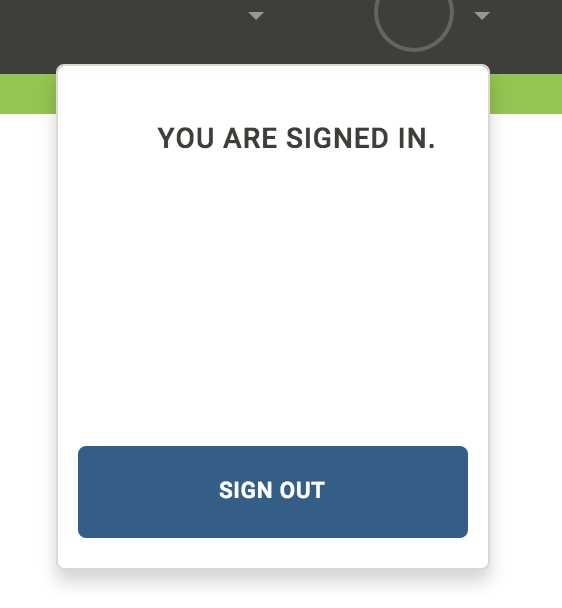
\includegraphics[width=0.4\textwidth]{figuras/architecture/accounts/logout/ui.png}
	\caption{Desvincular la cuenta de la aplicación.}
	\label{figure:architecture:accounts:logout:ui}
\end{figure}

\subsection{Recuperar contraseña}
Olvidar las contraseñas es algo recurrente. De hecho, más del 81\% a olvidado una contraseña utilizada en un sitio web \cite{online_berkeley_behavior_toward_password}. Esto demuestra lo importante que es contar con mecanismos de recuperación de contraseña.
El procedimiento es muy sencillo; se envía el \email usando el formulario de recuperación de contraseña(\refFigura{figure:architecture:accounts:reset:form}). El sitio genera una contraseña temporal y es enviada al correo.

\begin{figure}[H]
	\centering
	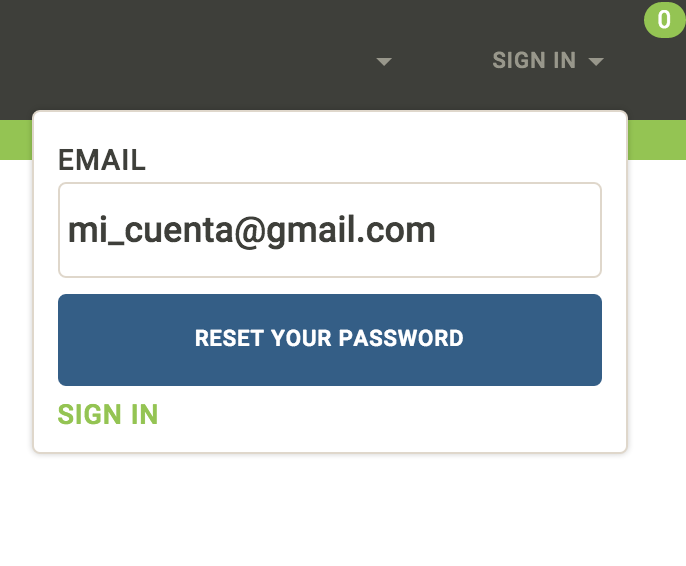
\includegraphics[width=0.4\textwidth]{figuras/architecture/accounts/reset/form.png}
	\caption{Formulario de restauración de contraseña.}
	\label{figure:architecture:accounts:reset:form}
\end{figure}

Las restricciones del formulario de recuperación de contraseña se ven en la \reftabla{tab:architecture:accounts:recovery:form}.

\begin{table}[H]
    \centering
	\begin{tabular}{ |l|c||l| }
		\hline Campo & Requerido & Restricción \\ \hline
		\multirow{2}{*}{\textit{Email Address}} &  \multirow{2}{*}{\checkmark}
				& - Debe ser un \email válido. \\ 
			& 	& - El \email debe estar en la base de datos. \\ \hline
	\end{tabular}
 	\caption{Resumen restrincciones para recuperación de contraseña.}
    \label{tab:architecture:accounts:recovery:form}
\end{table}

\subsection{\loginUpperCPT  con servicio de autenticación \thirdParty}
%\subsection{Autenticarse con proveedores de \oauthLoginINT }

La aplicación permite hacer \loginCPT a través de servicios de autenticación \thirdParty tales como \facebook, \googleNAME, \twitterNAME, \gitHubNAME, entre otros. En la \refFigura{figure:account:login:log_in_plus_facebook} se observa la existencia de un servicio \thirdParty para la autenticación en la aplicación.


\begin{figure}[H]
	\centering
	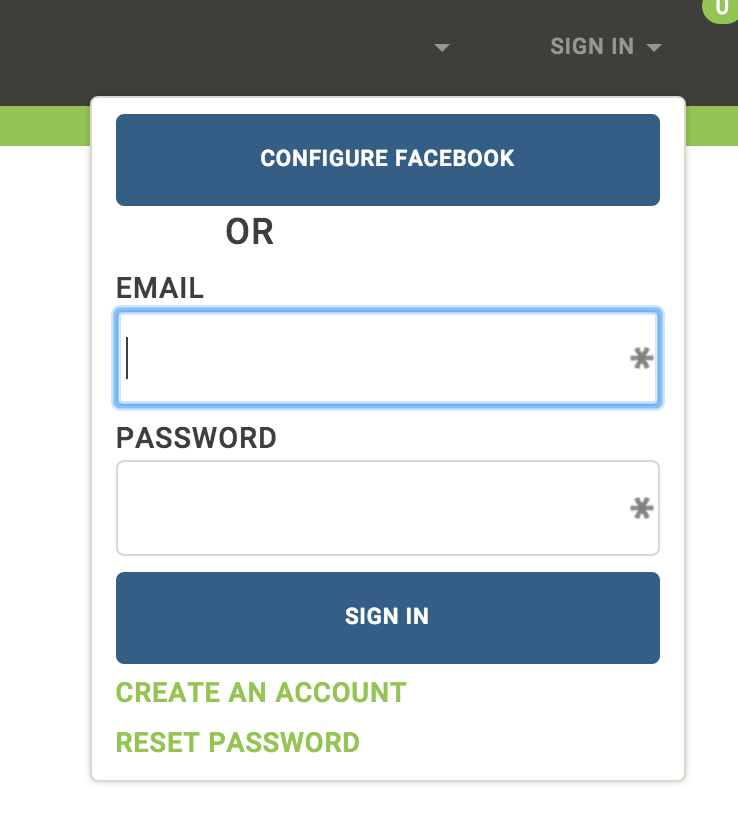
\includegraphics[width=0.4\textwidth]{figuras/architecture/accounts/login/log_in_plus_facebook.png}

	\caption{Autenticarse utilizando un servicio \thirdParty.}
	\label{figure:architecture:accounts:login:log_in_plus_facebook}
\end{figure}

%Es importante agregar que el sistema automáticamente agrega en la interfaz la opción de autenticarse utilizando el servicio \thirdParty simplemente agregando el \packagesAS de \meteorNAME; y por consiguiente este desaparecerá si el \packagesAS es removido. En la \refFigura{figure:architecture:accounts:login:log_in_all_package} se aprecian varios servicios \thirdParty para la autenticación de la aplicación.
Es importante destacar que el sistema permite agregar o esconder las opciones \thirdParty de la interfaz. En la \refFigura{figure:architecture:accounts:login:log_in_all_package} se ven los proveedores \oauthLoginINT \facebook, \gitHubNAME, \googleNAME, \twitterNAME respectivamente..

\begin{figure}[H]
	\centering
	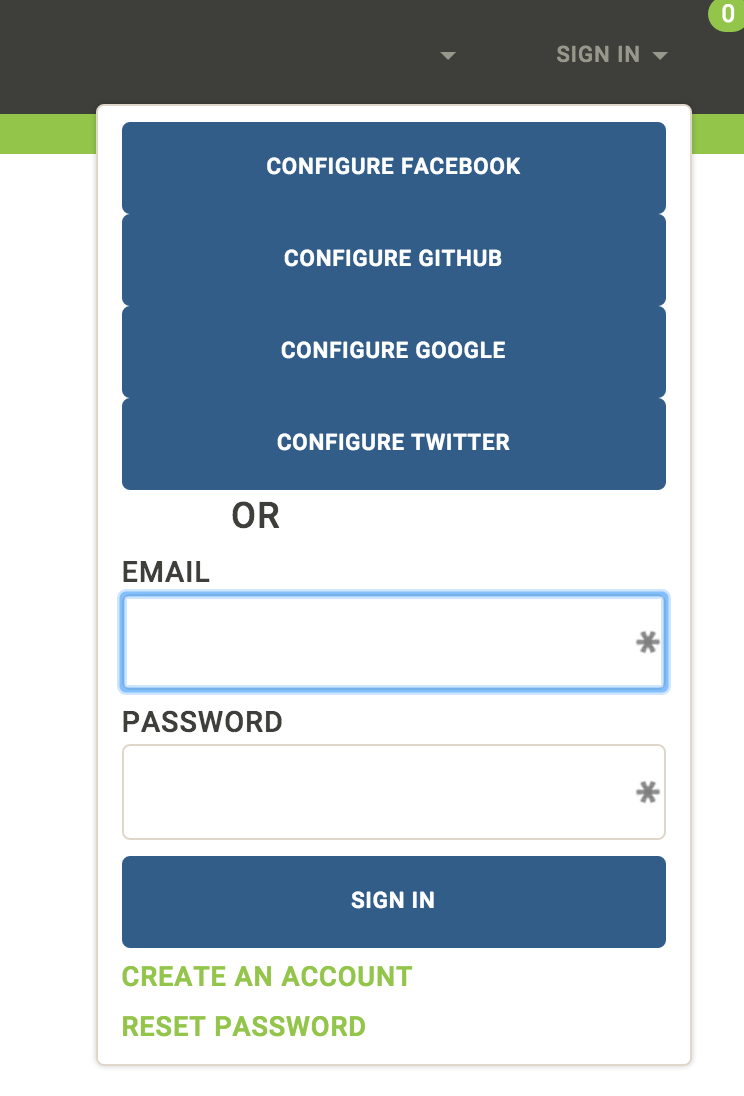
\includegraphics[width=0.4\textwidth]{figuras/architecture/accounts/login/log_in_all_package.png}

	\caption{Formulario de autenticación para utilizar uno de varios servios \thirdParty.}
	\label{figure:architecture:accounts:login:log_in_all_package}
\end{figure}